\chapter{State of the Art}
\label{cap:state-of-the-art}

\section{Self-Adaptive Software Systems}
\label{sec:sas}
In modern-day applications, software complexity has extremely increased thanks to the spread of highly available and faster wireless connection such as in the Internet of Things (IoT) ambit. Since software is often deployed in dynamic contexts, where requirements, environment assumptions and usage profiles vary continuously, software complexity increased over time to the point where it is often composed by a number of sub-components and/or sub-services that work together in order to offer a service to the users. This is the case of service-oriented applications -- also called Service Based Systems (SBS) -- that are composed by multiple \emph{services} and \emph{components}. In these systems, services offered by third-party providers are dynamically composed into workflows to deliver complex functionalities, so SBSs rely on self adaptation to cope with the uncertainties associated with third-party services as the loose coupling of services makes a reconfiguration feasible. Without adaptation, the application is prone to degraded performance  because of faulty components, messages lost between services or delays due to an increasing number of users.

During the past decade a lot of research has been made in this scope but the engineering of adaptive systems remains an incredible challenge\cite{soft-eng-for-sas-2}. In order to solve the problem, \textbf{Self-Adapting Software Systems (SASS)} are born. These are flexible systems that can adapt themselves to their contextual needs and can do so with the highest performance and availability. General discussion concerning the issue and the state of the art in the design and implementation have been presented\cite{soft-eng-for-sas-2}\cite{survey-aut-comp}\cite{self-adap-soft}\cite{soft-eng-for-sas-1}\cite{soft-eng-for-sas-3}\cite{arch-based-appr-to-sas}\cite{sas-quant-ver}.

These kind of systems have some fundamental properties called auto-managing that are:
\begin{itemize}
	\item Auto-configuration
	\item Auto-recovery in case of failure
	\item Auto-optimization
	\item Auto-protection
\end{itemize}
All these properties can be grouped in two more abstract concepts which are self-awareness and context-awareness.

\textbf{Self-Awareness} is the ability of the system to be able to monitor itself in terms of available resources and behavior.

\textbf{Context-Awareness} is the ability of the system to understand the environment where it is working, using the information provided by its components, and adapt itself to all the changes that can occur during its normal operational status.
To better understand how a SASS works we need to answer some simple questions:
\begin{itemize}
	\item Who is adapting?
	\item What adaptation is required?
	\item When is it necessary to adapt?
	\item Where is it needed to change something?
	\item Why is it needed an adaptation?
	\item How do we achieve this goal?
\end{itemize}

During the past years have been developed some dimensions that help to answer all this simple questions: \emph{Time}, \emph{Reason}, \emph{Level}, \emph{Technique} and \emph{Adaptation Control} shown in Figure \ref{fig:dimensions}.
\begin{figure}[ht]
	\centerline
	{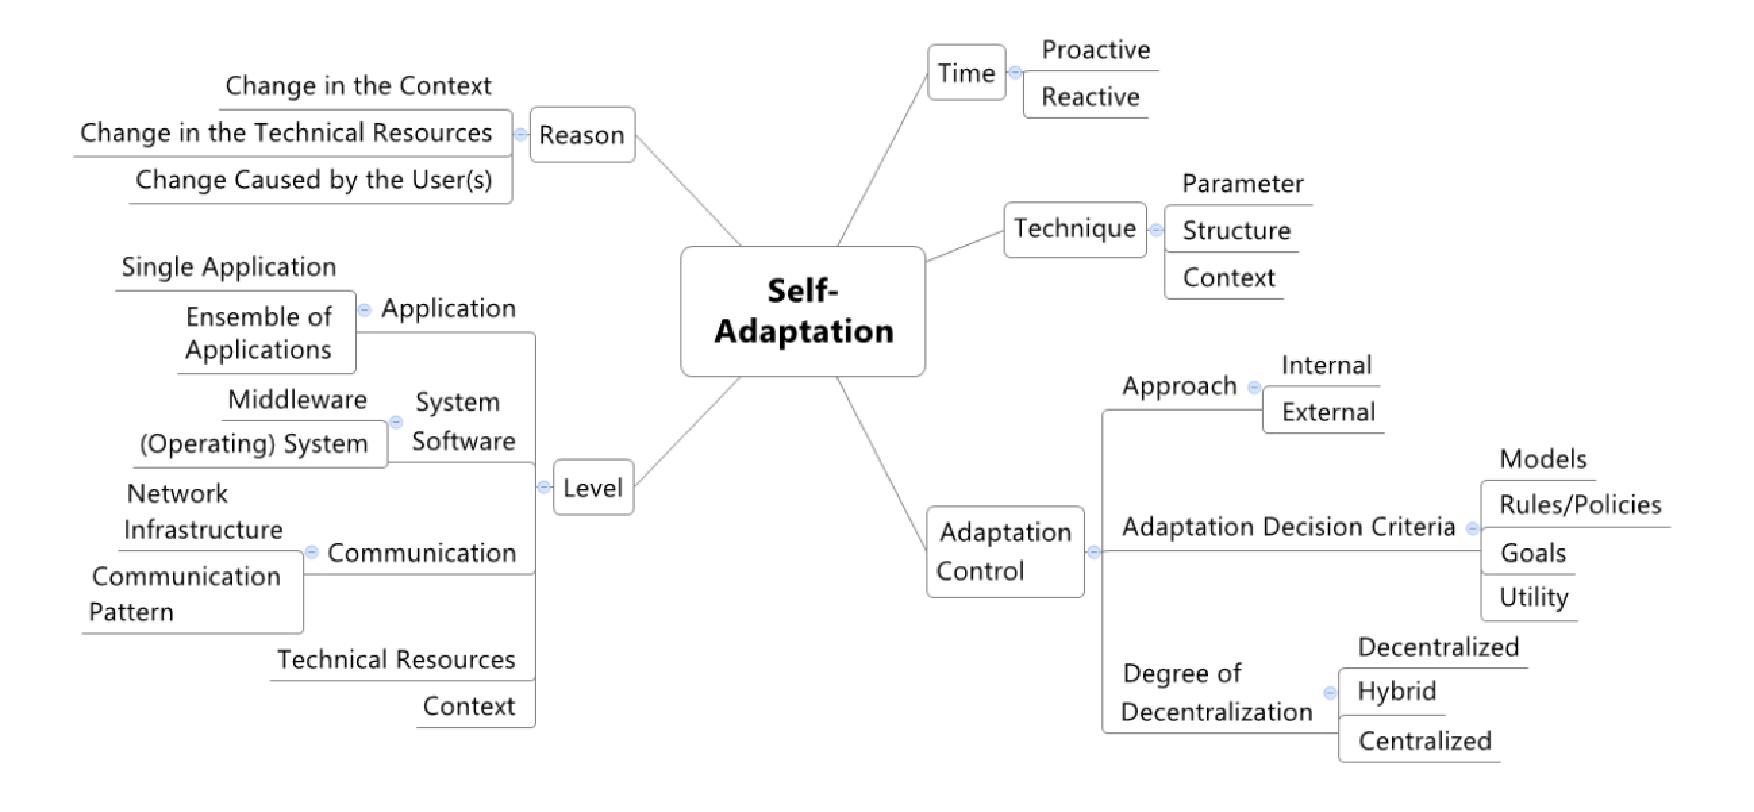
\includegraphics[scale=0.50]{img/dimensions.png}}
	\caption[The Dimensions]{The Dimensions to analyze adaptation.\cite{eng-appr-sas}}
	\label{fig:dimensions}
\end{figure}

\textbf{Who is adapting?} As the name suggests, it's the system itself that changes something in order to preserve some given constraint.

\textbf{What adaptation is required?} The \emph{Technique} dimension is the one that answers this question in fact the software engineer can change either the parameters or the system can be considered as a set of components. The former case allows to fine tuning the system at the expense of an higher complexity, the latter is called composite vision and permits the systems to cooperate exchanging algorithms and much more important, reusing components which improve performance because failed or defected components can be replaced.

\textbf{When it is necessary to adapt?} The \emph{Time} dimension is crucial in this situation. There are three typical approaches: the reactive one is the more traditional one which states that an adaptation is needed only after a causative event. The other two approaches are more interesting and they are predictive and proactive. The former studies the system before any event and calculate the need of an adaptation, the latter applies and adaptation despite an event and improves the performance. From the user perspective the proactive approach is the best because it doesn't interrupt the operation of the system in any load but it is the more complicated to implement. Monitoring continuously the system is a costly task to do, on the other side an adaptive monitoring is simple that analyze only specific aspect and/or resources and intervenes only if needed.

\textbf{Where it is needed to change something?} In general a SASS is composed by two main part: the the Adaptability Logic (AL) and the Managed Resource (MR). The former in general doesn't change, the latter is composed at the base of the hardware and of the software such as the operating system or, in case of distributed systems, the middleware that control the hardware; at a higher level of the application. These are the parts that require adaptation. To answer this question is needed to decide at which level the operation has to be applied without neglecting the relationship between the MR and the AL which is composed by the network that connects them and/or the view of the communication patterns. Thus \emph{Level} is the considered dimension.

\textbf{Why it is needed an adaptation?} In this case, \emph{Reason} is the right dimension. There can be one or more reason because a system needs adaptation such as a change in the available resources, a change in the environment or a change in the user base of the system.

\textbf{How do we achieve this goal?} The answer to this question is more complicated than the others because it needs a new topic called \emph{Adaptation Control}.

\subsection{Adaptation Control}
In the literature can be found 2 approaches: the \emph{internal approach} that intertwine the adaptation logic with the system resources, which has problems with the maintainability and scalability of the system, and the \emph{external approach} that splits the system into adaptation logic and managed resources, which increases maintainability and scalability through modularization.

The control unit needs a metric in order to decide how to adapt and in literature different metrics are present: models, rules and policies, goal or utility functions \cite{autonomic-computing}.

Another aspect of the adaptation logic is the degree of decentralization. If we have a system with limited resources then a centralized adaptation logic has to be preferred but with greater systems a decentralized AL can improve performance and  every sub-system can communicate with another with different patterns of communication. Of course hybrid technique can be made mixing the previous approaches.

\subsubsection{Adaptation Logic Issues}
As said before a SASS is composed of managed resources and the adaptation logic; it can be represented by the tuple \texttt{SASS = (AL, MR)}. \emph{AL = $a_1$, \dots, $a_n$}, with $a_i$ representing a logic element,  monitors the environment (M), analyzes the data for change (A), plans adaptation (P) and control the execution of the adaptation (E): these are known as \emph{MAPE cycle} or \emph{MAPE functionality}\cite{vision-aut-comp}. \emph{MR = $mr_1$, \dots, $mr_n$}, with $mr_i$ representing a resource, is the set of resources such as hardware with software, smart-phones, robotics or unmanned vehicles. Figure \ref{fig:sass} shows a SASS where the dashed line represent the system border.
\begin{figure}[ht]
	\centerline
	{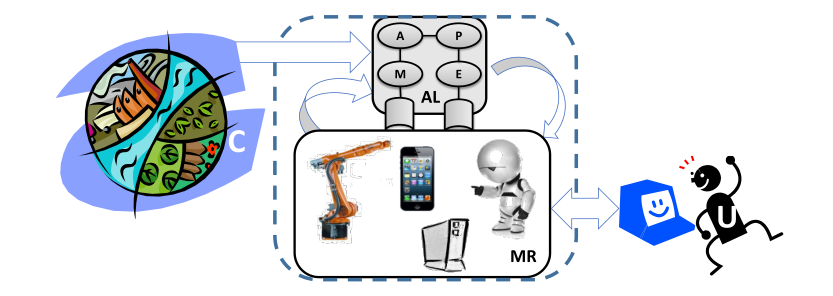
\includegraphics[scale=0.55]{img/managed-resources.png}}
	\caption[A SASS]{A SASS (AL = Adaptation Logic, MR = Managed Resources, U = User(s), C = Context, M,A,P,E = MAPE functionality).\cite{eng-appr-sas}}
	\label{fig:sass}
\end{figure}
The dimension can therefore be mapped to the MAPE functionalities as shown in table \ref{tab:mape}.
\begin{table}[ht!b]
	\centering
	\begin{tabular}{|l||p{2.4cm}|p{2.4cm}|p{2.4cm}|p{2.4cm}|}
		\hline 
		& \textbf{Time} & \textbf{Reason} & \textbf{Level} & \textbf{Technique} \\ 
		\hline 
		\textbf{Monitoring} & Continuos & What to monitor & Identification of the levels & --- \\ 
		\hline 
		\textbf{Analyzing} & Algorithms depend on reactive or proactive dimension & Where to analyze & --- & --- \\ 
		\hline 
		\textbf{Planning} & --- & What should be influenced by planning & Adaptation plans address these levels & Plans for performing the techniques \\ 
		\hline 
		\textbf{Executing} & --- & --- & Execution of the change on the levels & Execution of the change on the levels \\ 
		\hline 
	
	\end{tabular} 
\caption[MAPE and Dimensions]{Relation of the MAPE Activities and the Dimensions}
\label{tab:mape}
\end{table}

\section{The SOLAR Framework}
\label{sec:solar-framework}
Working on the adaptability of a system can impact other quality attributes such as performance, reliability or maintainability and in the worst case improving adaptability can decrease part, if not all, of these attributes as stated in \cite{bass2003software}: \emph{quality attributes can never be achieved in isolation, the achievement of any one will have an effect, sometimes positive and sometimes negative, on the achievement of others}.

Find a balance between these quality attributes is often a challenging task because sometimes they're conflicting each other, e.g. lower cost and higher availability, so find an adaptability value that can meet all the requisites is, as a consequence, a challenging task too.

The SOLAR (SOftware quaLities and Adaptability Relationships) framework \cite{solar} helps the software architect to select the best set of components in order to fulfill the requirements trying to achieve a minimum level for some quality attribute such as availability and/or cost. This tool helps the software architect to build a suitable architecture for his needs but is not a \emph{"solution for every situation"}.

\subsection{The SOLAR Metrics}
\label{subsec:solar-metrics}
All the metrics in SOLAR are greatly inspired by \cite{po-metrics} and are all defined at an architecture level and static perspective. 

To define them, the software architecture relies on a component-and-connector view (C\&C view). In this C\&C view \emph{components} are principal computational elements present at runtime. The representation used in Figure \ref{fig:comp-example} uses the UML diagram and shows some components and their respective connections.

\begin{figure}[ht]
	\centerline
	{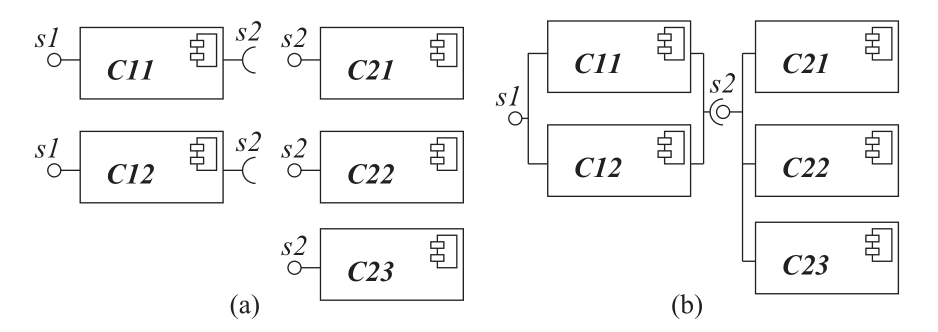
\includegraphics[scale=0.55]{img/solar-comp-example.png}}
	\caption[SOLAR Components Example]{(a) A set of components and their interfaces and (b) the C\&C view of the components in (a)\cite{solar}.}
	\label{fig:comp-example}
\end{figure}

Components have interfaces attached to ports. \emph{Connectors} are pathways of interaction between components and also have interfaces or roles. In Figure \ref{fig:solar-arch-example} it is shown an example of an architecture, the used components are highlighted in gray; this example will be used to explain the metrics later in this chapter.

\begin{figure}[ht]
	\centerline
	{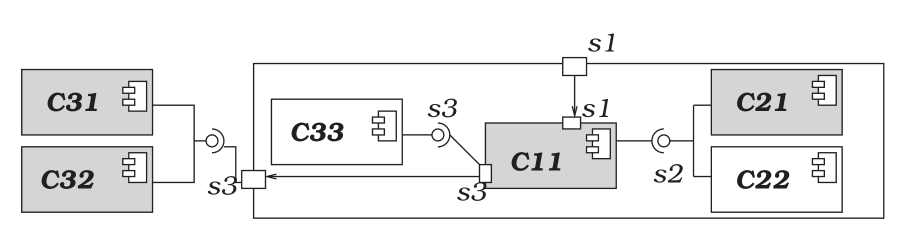
\includegraphics[scale=0.55]{img/solar-arch-example.png}}
	\caption[SOLAR Example Architecure]{C\&C view: discovered components and used components (in gray).\cite{solar}}
	\label{fig:solar-arch-example}
\end{figure}

In the architecture of Figure \ref{fig:solar-arch-example}:
\begin{itemize}
	\item the service S1 is provided by component C11 that is unique and must be in use. S1 is the provided service of this architecture.
	\item component C11 requires S2 and S3 services.
	\item service S2 is provided by C21 and C22 where only C21 is in use.
	\item service S3 is provided by C31, C32 and C33 but only C31 and C32 are in use.
\end{itemize}

\subsubsection{Absolute adaptability of a service (AAS)}
This metric measures the number of used components for providing a given service.
\[ AAS \in \mathbb{N}^n |AAS_i = |UC_i|\]
Quantifies how much adaptable a service is by counting the different alternatives to execute the service (1 no adaptable, $>$1 adaptable), where the service adaptability grows according to the number of components able to provide it. 

\noindent Referring to the example in Figure \ref{fig:solar-arch-example}, we observe that $AAS = [1, 1, 2]$.

\subsubsection{Relative adaptability of a service (RAS)}
This metric measures the number of used components that provide a given service with respect to the number of components actually offering such service.
\[ RAS \in \mathbb{Q}^n | RAS_i = \frac{|UC_i|}{|C_i|} \]
It describes how each service stresses its adaptability choices and it informs how much more adaptable the service could be. RAS vector values near to one mean that the service is using almost all the adaptability potentially reachable. 

\noindent Referring to the example in Figure \ref{fig:solar-arch-example}, we observe that $RAS = [1, 0.5, 0.6]$.

\subsubsection{Mean of absolute adaptability of services (MAAS)}
This metric measures the mean number of used components per service.
\[ MAAS \in \mathbb{Q} | MAAS = \frac{\sum_{i=1}^{n} AAS_i}{n}  \]
It offers insights into the mean size and effort needed to manage each service.

\noindent Referring to the example in Figure \ref{fig:solar-arch-example}, $MAAS = 4/3 = 1.3$. 

Architectures with more adaptable services have higher values of MAAS. Besides, a $MAAS > 1$ means that the architecture includes adaptable services (at least one of the components $AAS_i > 1$). For $MAAS \le 1$, there may be adaptable services or not (AAS should be checked in this case).

\subsubsection{Mean of relative adaptability of services (MRAS)}
This metric represents the mean of RAS.
\[ MRAS \in \mathbb{Q} | MRAS = \frac{\sum_{i=1}^{n}RAS_i}{n}\]
It informs about the mean utilization of the potential components for each service. Values of this metric range between zero and one.

\noindent Referring to the example, $MRAS = (1 + 0.5 + 0.6)/3 = 0.72$.

The higher the MRAS of an architecture, the more adaptable its services are, on average. The maximum value of this metric is obtained when $RAS_i = 1 \;\;\forall i \in [1, \dots, n]$, which is in turn obtained when all services are as much adaptable as possible because they use all the available components. Therefore, a value close to one for MRAS means that, on average, services are as much adaptable as possible. A value close to zero means that: 
\begin{enumerate}
	\item[\textbf{a)}] services can be much more adaptable (adding components not yet used)
	\item[\textbf{b)}] different architecture alternatives with the same quantity of adaptability can be created
\end{enumerate}

\subsubsection{Level of system adaptability (LSA)}
This metric measures the number of components used to make up the system with respect to the number of components that the most adaptable architecture would use.
\[ LSA \in \mathbb{Q}{0..1} | LSA = \frac{\sum_{i=1}^{n}AAS_i}{\sum_{i=1}^{n}|C_i|} \]
The value of this metric ranges between zero and one. For LSA, a value of one means that the system is using all existing components for each service, i.e., $AAS_i = |C_i | \forall i \in {1,\dots, n}$, and then its adaptability is already to the maximum. A value close to one means that the market offers few choices to increase the system architectural adaptability. When a new component is bounded to the architecture, LSA increases in a constant value ($1/\sum{{i=1}^{n}|C_i}$) irrespective of the number of components already considered for the same service.

\noindent Referring to the example in Figure \ref{fig:solar-arch-example}, $LSA = 4/(1 + 2 + 3) = 0.6$.

Table \ref{tab:solar-metrics-summary} summarizes the five metrics and their values for the example in Figure \ref{fig:solar-arch-example}.

\begin{table}[ht!b]
	\centering
	\begin{tabular}{|l|l|l|l|}
		\hline 
		Name & Range & Value & Example in Fig. \ref{fig:solar-arch-example} \\ 
		\hline 
		AAS & $\mathbb{N}^n$ & ${|UC_i|}$ & $[1,1,2]$ \\

		RAS & $\mathbb{Q}^n \in {0,\dots,1}$ & ${\frac{|UC_i|}{|C_i|}}$ & $[1,0.5,0.6]$ \\ 

		MAAS & $\mathbb{Q}_+$ & $\frac{\sum_{i=1}^{n}AAS_i}{n}$ & $1.3$ \\ 

		MRAS & $\mathbb{Q}^n \in {0,\dots,1}$ & $\frac{\sum_{i=1}^{n}RAS_i}{n}$ & $0.72$ \\ 
		
		LSA & $\mathbb{Q}^n \in {0,\dots,1}$ & $\frac{\sum_{i=1}^{n}AAS_i}{\sum_{i=1}^{n}|C_i|}$ & $0.6$ \\
		\hline 
		
	\end{tabular} 
	\caption[SOLAR Metrics]{Summary of the metrics.\cite{solar}}
	\label{tab:solar-metrics-summary}
\end{table}

\subsection{Relating adaptability to a system quality attribute}
The analysis of the relation between system adaptability and quality attributes can give three different results as shown in Table \ref{tab:adapt-qual}.  In the rows we read that, when the adaptability increases then some quality attributes:
\begin{itemize}
	\item tend to increase their measured values
	\item tend to decrease their measured values
	\item are not affected. We are not interested in this group since we are focussed on the influence of adaptability on the requirement.
\end{itemize}

\noindent The columns in the table consider how the quality requirement is formulated:
\begin{itemize}
	\item as higher than, e.g., "system availability shall be higher than\dots"
	\item as lower than, e.g., "system mean response time shall be lower than\dots"
\end{itemize}

Each region of interest in Table \ref{tab:adapt-qual} has been labeled as Helps or Hurts to indicate the effect of the adaptability upon the quality requirement. 

\noindent The best cases are when the quality attribute completely depends on the adaptability such as:
\begin{enumerate}
	\item The higher the adaptability, the higher the quality attribute
	\item The lower the adaptability, the lower the quality attribute
\end{enumerate}

In Figure \ref{fig:solar-inter-cases} are shown all the intermediate cases that can result mixing the two extreme cases above. The \emph{X} axis represents the adaptability value, The \emph{Y} axis represent the quality attribute. For each value of adaptability there are two extreme values:
\begin{itemize}
	\item $Q_{A_iU}$ is the maximum value of the quality attribute with respect to $A_i$
	\item $Q_{A_iL}$ is the minimum value of the quality attribute with respect to $A_i$
\end{itemize} 
Between these extreme values there are all the architecture that have the same adaptability and intermediate quality attribute value. Among all the $Q_{A_iU}$ and $Q_{A_iL}$ in the graph, two of them have a particular meaning: $Adapt^+$ and $Adapt^-$.

To describe the meaning of $Adapt^-$ and $Adapt^+$ we focus on parts (a) and (d) in Figure \ref{fig:solar-inter-cases}. $Adapt^-$ is the lowest $A_i$ for which we can find an architecture satisfying the requirement. $Adapt^+$ is the lowest $A_i$ whose bounds, $Q_{A_iU}$ and $Q_{A_iL}$, satisfy the requirement. These values indicate that to fulfill the requirement, the architecture must have at least adaptability $Adapt^-$, and, any architecture with at least $Adapt^+$ will also satisfy it. For adaptabilities between them, there will be architectures satisfying the requirement (those highlighted in the figure) and others that will not. 

In parts (b) and (c) in Figure \ref{fig:solar-inter-cases} (regions where the adaptability Hurts), $Adapt^-$ is the threshold adaptability value for which any architecture with adaptability $A_i \le Adapt^-$ fulfills the requirement; and $Adapt^+$ is the maximum $A_i$ for which we know that exists some architecture that satisfies the requirement.

\begin{table}[ht!b]
	\centering
	\begin{tabular}{lx{3cm}x{3cm}}
		\firsthline
		\multirow{2}{*}{When adaptability increases} & \multicolumn{2}{c}{Requirement formulated as} \\
		\cline{2-3}
		& \emph{Higher than} & \emph{Lower than} \\
		\hline
		The quality attribute value increases & Helps & Hurts \\
		The	quality attribute value decreases & Hurts & Helps \\
		The	quality attribute is not affected & \multicolumn{2}{c}{No effect}\\
		\hline
	\end{tabular}
	\caption[Adaptability w.r.t. Quality Requirements]{Effect of adaptability on a measured quality requirement.\cite{solar}}
	\label{tab:adapt-qual}
\end{table}
\begin{figure}[ht]
	\centerline
	{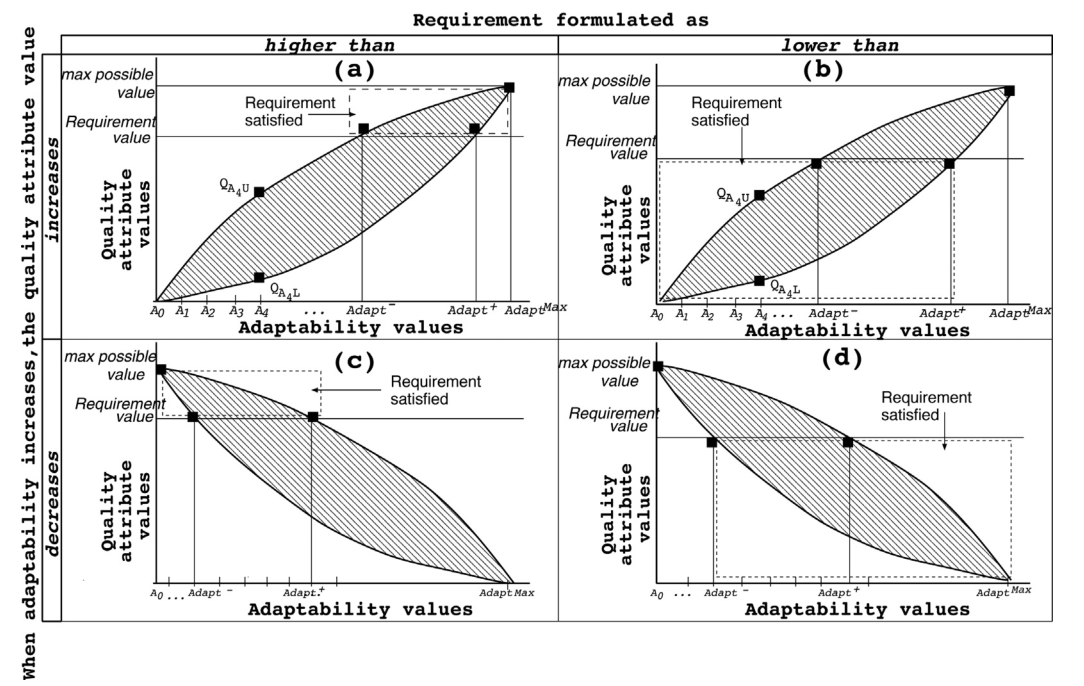
\includegraphics[scale=0.55]{img/solar-inter-cases.png}}
	\caption[Relations among Adaptability and Other Quality attributes.]{Relations among adaptability and other quality attributes.\cite{solar}}
	\label{fig:solar-inter-cases}
\end{figure} 
\subsection{Analysis of the approach and its limits}
Both of these tools want to help the software architect in choosing the right set of components in order to satisfy the adaptability requirements and if possible other quality attributes. With the SOLAR framework all the possible architectures that satisfy the requisites are generated and the choice is left to the architect. This approach is for sure slower but is a valid tool to have an idea of the possible outcome and build an architecture from scratch. On the other side it presents some limitations presented in no particular order:
\begin{itemize}
	\item It analyzes all the architecture only with a static analysis using the component diagram.
	\item All components are given equal importance thus the time a component is used and the number of usages per call is completely ignored.
	\item It does not considers the probability of failure of a component at runtime.
	\item Requires a lot of time to produce complete results.
\end{itemize}
In the next chapter it is shown how to analyze the quality of a software and in particular how to evaluate the adaptability of a software with respect to some attributes such as cost and availability.